% Multi-panel figure generated by plot_experiment2_metrics_modelbased.py.
% Requires \usepackage{graphicx} and \usepackage{subcaption}. Paths are
% relative to the repo root (Figs/...); adjust \graphicspath or the paths
% below to match the Overleaf project.
% Include with: % Multi-panel figure generated by plot_experiment2_metrics_modelbased.py.
% Requires \usepackage{graphicx} and \usepackage{subcaption}. Paths are
% relative to the repo root (Figs/...); adjust \graphicspath or the paths
% below to match the Overleaf project.
% Include with: % Multi-panel figure generated by plot_experiment2_metrics_modelbased.py.
% Requires \usepackage{graphicx} and \usepackage{subcaption}. Paths are
% relative to the repo root (Figs/...); adjust \graphicspath or the paths
% below to match the Overleaf project.
% Include with: % Multi-panel figure generated by plot_experiment2_metrics_modelbased.py.
% Requires \usepackage{graphicx} and \usepackage{subcaption}. Paths are
% relative to the repo root (Figs/...); adjust \graphicspath or the paths
% below to match the Overleaf project.
% Include with: \input{Figs/multifigure/experiment2_modelbased_nmse_true_figure}
\begin{figure}[htbp]
\centering
\begin{subfigure}[t]{0.48\linewidth}
  \centering
  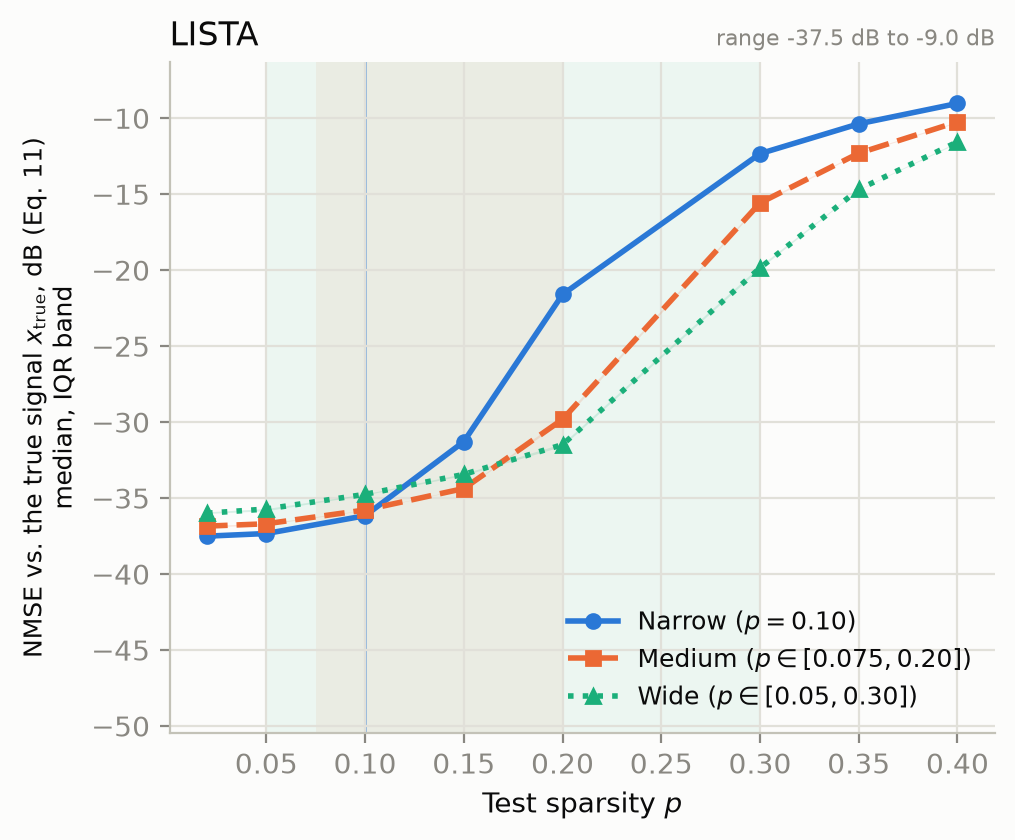
\includegraphics[width=\linewidth]{Figs/experiment2/experiment2_modelbased_nmse_true_lista.png}
  \caption{LISTA}
  \label{fig:experiment2-modelbased-nmse-true-lista}
\end{subfigure}\hfill
\begin{subfigure}[t]{0.48\linewidth}
  \centering
  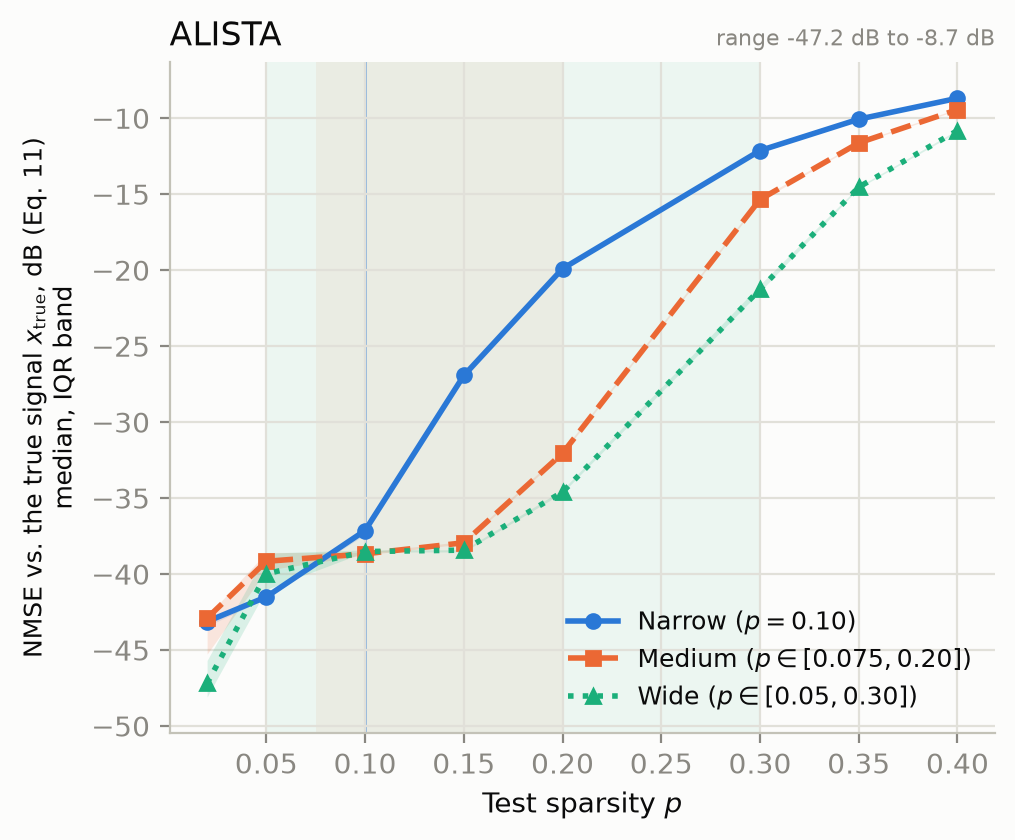
\includegraphics[width=\linewidth]{Figs/experiment2/experiment2_modelbased_nmse_true_alista.png}
  \caption{ALISTA}
  \label{fig:experiment2-modelbased-nmse-true-alista}
\end{subfigure}
\caption{NMSE vs. the true signal $x_\mathrm{true}$, dB (Eq. 11) vs.\ test sparsity $p$, $(m,n) = (210, 300)$, SNR 40 dB, 32 000 training instances, 10 seeds. Median over seeds with IQR band; one curve per training-sparsity width, with each width's training support shaded in its colour and the fixed narrow training point marked by a vertical line. Both panels share the y-axis; each panel's own data range is stated in its top-right corner.}
\label{fig:experiment2-modelbased-nmse-true}
\end{figure}

\begin{figure}[htbp]
\centering
\begin{subfigure}[t]{0.48\linewidth}
  \centering
  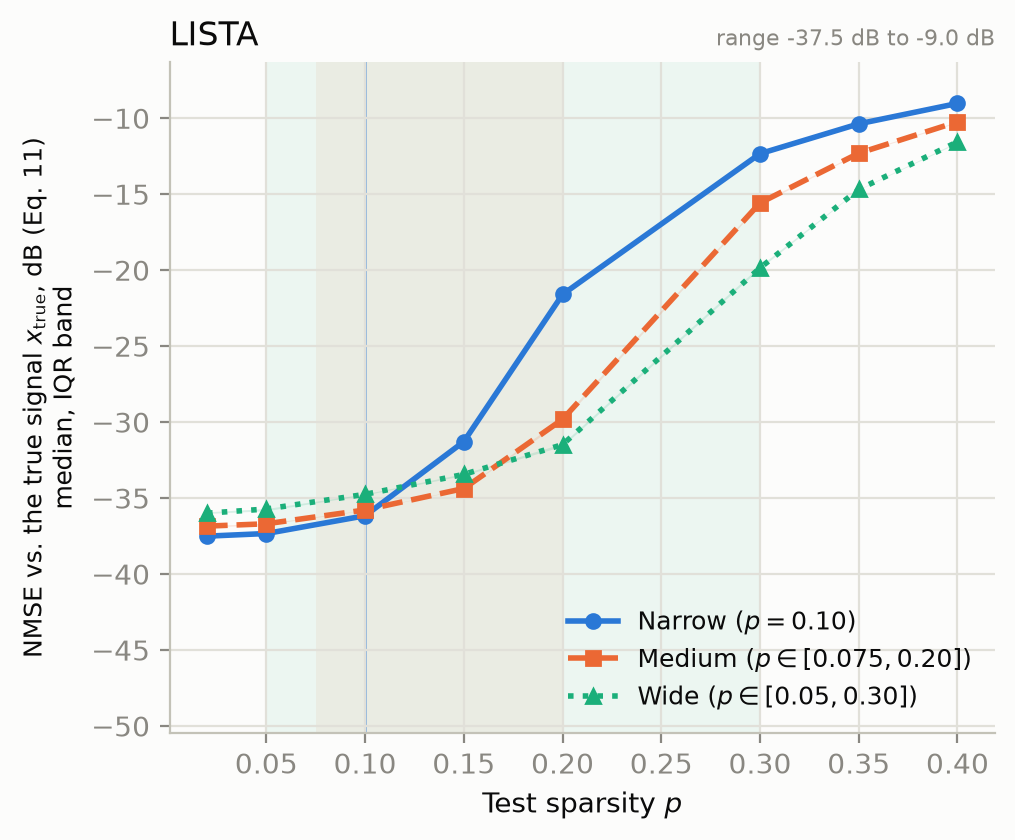
\includegraphics[width=\linewidth]{Figs/experiment2/experiment2_modelbased_nmse_true_lista.png}
  \caption{LISTA}
  \label{fig:experiment2-modelbased-nmse-true-lista}
\end{subfigure}\hfill
\begin{subfigure}[t]{0.48\linewidth}
  \centering
  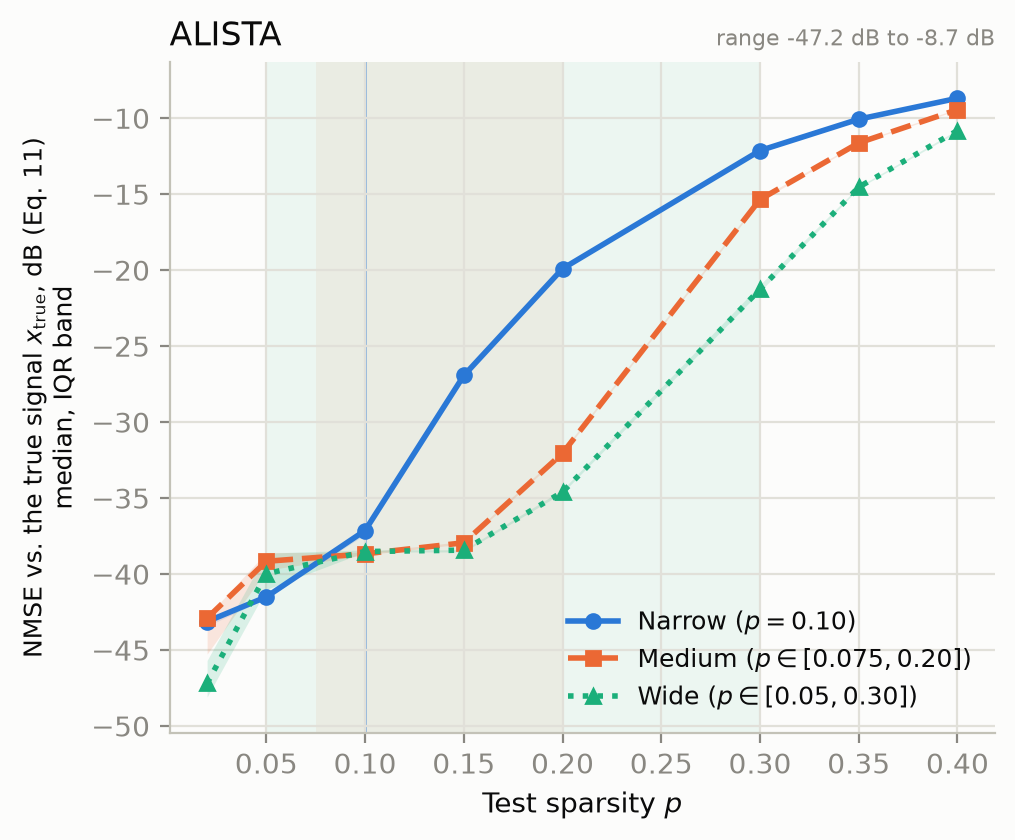
\includegraphics[width=\linewidth]{Figs/experiment2/experiment2_modelbased_nmse_true_alista.png}
  \caption{ALISTA}
  \label{fig:experiment2-modelbased-nmse-true-alista}
\end{subfigure}
\caption{NMSE vs. the true signal $x_\mathrm{true}$, dB (Eq. 11) vs.\ test sparsity $p$, $(m,n) = (210, 300)$, SNR 40 dB, 32 000 training instances, 10 seeds. Median over seeds with IQR band; one curve per training-sparsity width, with each width's training support shaded in its colour and the fixed narrow training point marked by a vertical line. Both panels share the y-axis; each panel's own data range is stated in its top-right corner.}
\label{fig:experiment2-modelbased-nmse-true}
\end{figure}

\begin{figure}[htbp]
\centering
\begin{subfigure}[t]{0.48\linewidth}
  \centering
  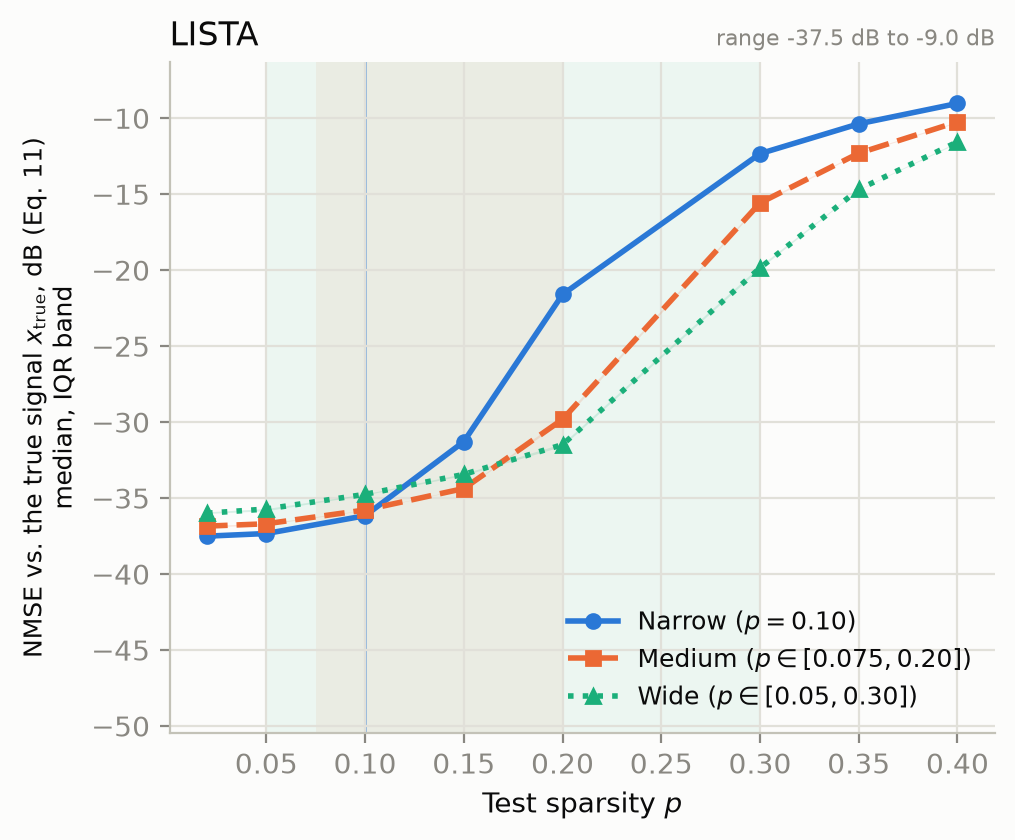
\includegraphics[width=\linewidth]{Figs/experiment2/experiment2_modelbased_nmse_true_lista.png}
  \caption{LISTA}
  \label{fig:experiment2-modelbased-nmse-true-lista}
\end{subfigure}\hfill
\begin{subfigure}[t]{0.48\linewidth}
  \centering
  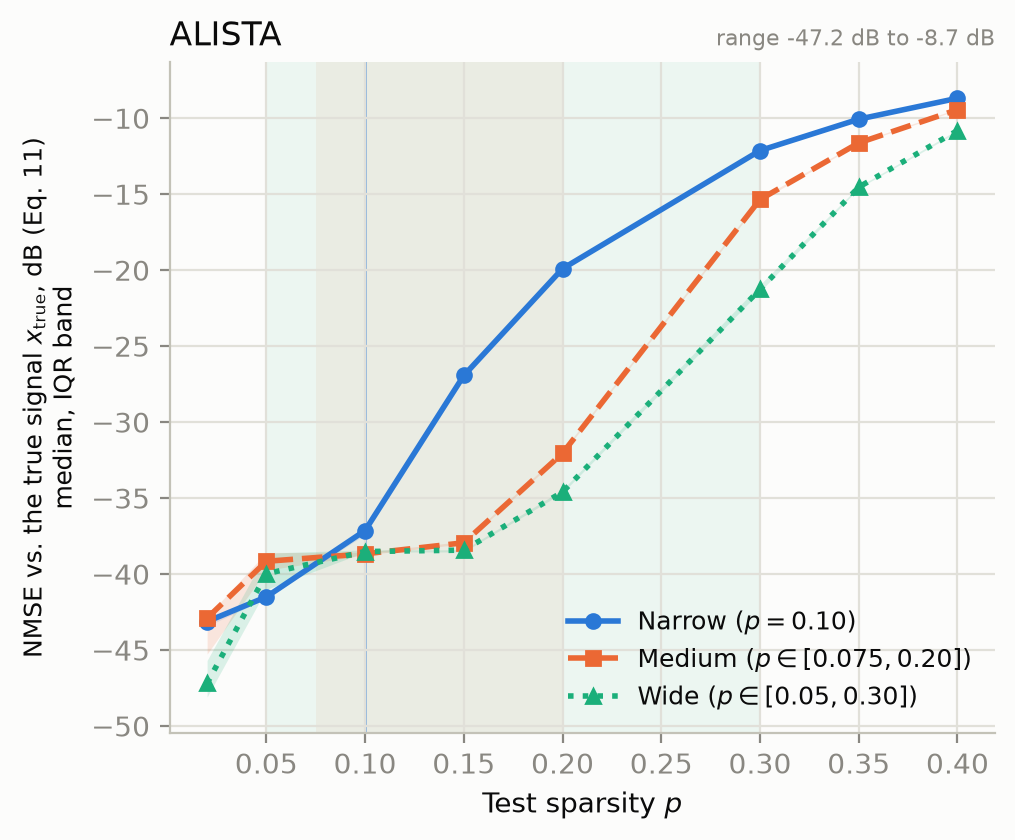
\includegraphics[width=\linewidth]{Figs/experiment2/experiment2_modelbased_nmse_true_alista.png}
  \caption{ALISTA}
  \label{fig:experiment2-modelbased-nmse-true-alista}
\end{subfigure}
\caption{NMSE vs. the true signal $x_\mathrm{true}$, dB (Eq. 11) vs.\ test sparsity $p$, $(m,n) = (210, 300)$, SNR 40 dB, 32 000 training instances, 10 seeds. Median over seeds with IQR band; one curve per training-sparsity width, with each width's training support shaded in its colour and the fixed narrow training point marked by a vertical line. Both panels share the y-axis; each panel's own data range is stated in its top-right corner.}
\label{fig:experiment2-modelbased-nmse-true}
\end{figure}

\begin{figure}[htbp]
\centering
\begin{subfigure}[t]{0.48\linewidth}
  \centering
  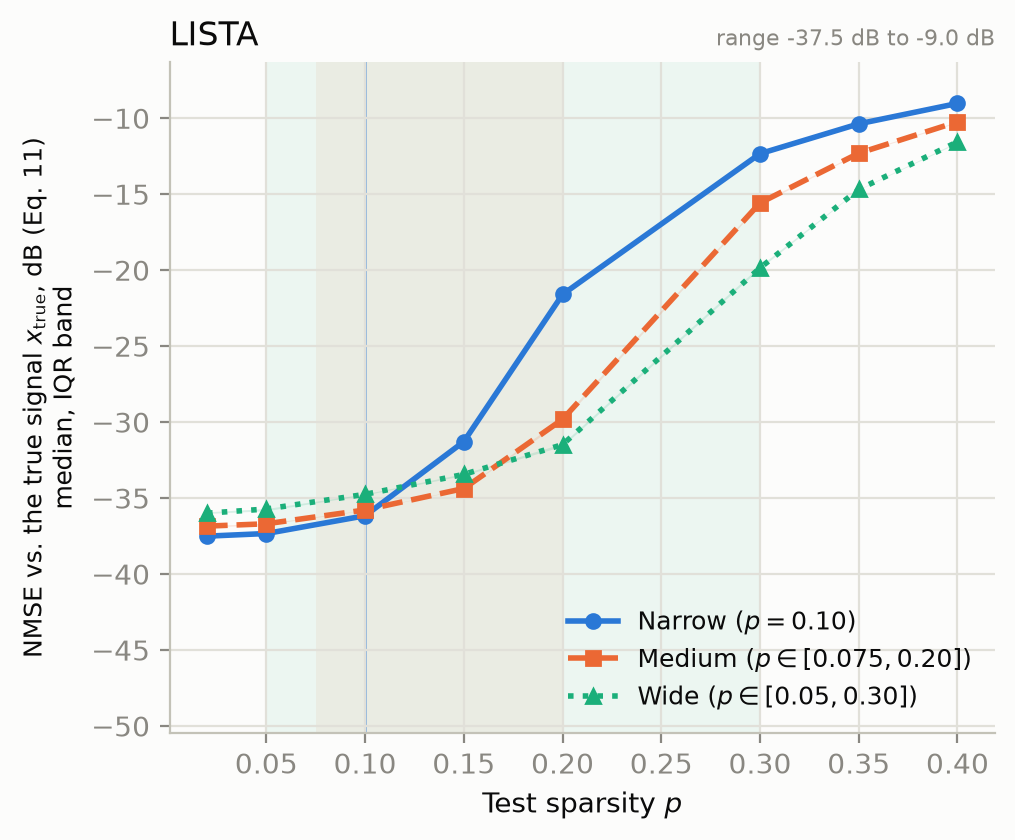
\includegraphics[width=\linewidth]{Figs/experiment2/experiment2_modelbased_nmse_true_lista.png}
  \caption{LISTA}
  \label{fig:experiment2-modelbased-nmse-true-lista}
\end{subfigure}\hfill
\begin{subfigure}[t]{0.48\linewidth}
  \centering
  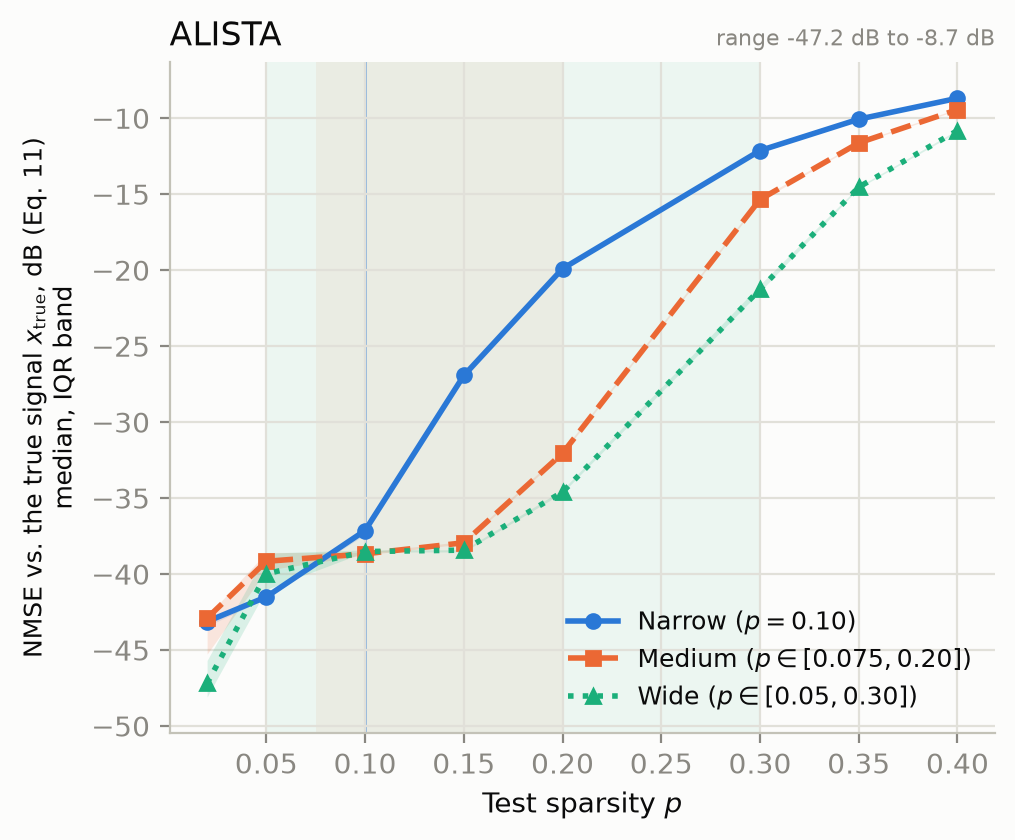
\includegraphics[width=\linewidth]{Figs/experiment2/experiment2_modelbased_nmse_true_alista.png}
  \caption{ALISTA}
  \label{fig:experiment2-modelbased-nmse-true-alista}
\end{subfigure}
\caption{NMSE vs. the true signal $x_\mathrm{true}$, dB (Eq. 11) vs.\ test sparsity $p$, $(m,n) = (210, 300)$, SNR 40 dB, 32 000 training instances, 10 seeds. Median over seeds with IQR band; one curve per training-sparsity width, with each width's training support shaded in its colour and the fixed narrow training point marked by a vertical line. Both panels share the y-axis; each panel's own data range is stated in its top-right corner.}
\label{fig:experiment2-modelbased-nmse-true}
\end{figure}
